\newpage
%
% Návrh systému na tvorbu poznámok
%
\ifthenelse {\boolean{bachelor}}
{
	%\section{Design}
	\section{Návrh systému na tvorbu poznámok}
}
{
	%\chapter{Design}
	\chapter{Návrh systému na tvorbu poznámok}
}
\label{design}
Systém na tvorbu poznámok vyžaduje splnenie viacerých požiadaviek. Hlavné z nich sú vytvorenie poznámky a možnosť jej následnej interaktívnej úpravy. Ďalej sú to tvorba viacnásobných poznámok, vytváranie poznámok na základe pravidiel s využitím závislostí slov, ktoré môžu byť aplikované na viacero viet, výber vhodnej databázy s adekvátne vytvoreným databázovým modelom. Spomenuté požiadavky sú opísané v nasledujúcich častiach.

%
% Tvorba poznámok
%
\ifthenelse {\boolean{bachelor}}
{
	%\subsection{Subsection}
	\subsection{Tvorba poznámok}
}
{
	%\section{Subsection}
	\section{Tvorba poznámok}
}
\label{subsection:notes_creation}
Pri spracovávaní viet potrebné extrahovať dôležité a konkrétne informácie, v našom prípade slová, a z extrahovaných informácií vytvoriť poznámku. Poznámka je zložená výhradne zo slov obsiahnutých vo vete, z ktorej bola vytvorená. Tým zabezpečíme, že poznámka nebude obsahovať irelevantné informácie z hľadiska vzťahu ku vete. 

Spracovávané vety sa môžu opakovať, a preto je dôležité, aby sa rovnaké a podobné vety spracovali vždy takým istým spôsobom. Pre tento účel je vhodné mať definované pravidlo (viď.~\fullref{subsubsection:rule_for_processing}), ktoré bude určovať, ako sa má daná veta spracovať. Aplikovaním pravidla na vetu vytvoríme poznámku. Používateľ má možnosť interaktívne upraviť poznámku, a tým pádom aj pravidlo, ktoré bolo použité na vytvorenie danej poznámku, v takom rozsahu, že sa vytvorená poznámka zmení podľa vykonaných zmien. Zmeny v pravidle sa musia prejaviť aj pri nasledujúcom aplikovaní pravidla na rovnakú alebo podobnú vetu. Používateľovi to poskytne kontrolou nad spôsobom, akým sa vytvárajú poznámky a bude si ich vedieť prispôsobiť - personalizovať.

%
% Pravidlo na spracovanie
%
\ifthenelse {\boolean{bachelor}}
{
	\subsubsection{Pravidlo na spracovanie}
}
{
	\subsection{Pravidlo na spracovanie}
}
\label{subsubsection:rule_for_processing}
Pravidlo na spracovanie určuje, ktoré informácie vo vete sú relevantné a majú byť použité v poznámke. Okrem určenia relevantnosti slov pravidlo taktiež určuje, na ktorej pozícií sa má konkrétna informácia vo výslednej poznámke nachádzať. Výsledná poznámka sa nemusí skladať iba z jednej vety, ale môže pozostávať z ľubovolného počtu viet. Počet viet, z ktorých bude poznámka pozostávať a miesta, na ktorých má byť pôvodná poznámka rozdelená na vety určuje pravidlo.

Skladá sa primárne zo štruktúry, ktorá je zložená najmä zo závislostí. Viac informácií o štruktúre je v časti~\fullref{subsection:structure_of_sentences_and_rules}. Okrem štruktúry obsahuje aj informácie o pozíciách, na ktorých sa má výsledná poznámka rozdeliť na menšie časti - vety.
%zo závislostí slov, ktoré sa majú nachádzať v poznámke. Pomocou závislosti vieme jednoznačne identifikovať a extrahovať konkrétne slovo z vety a pridať ho do poznámky. Okrem závislostí obsahuje aj informácie o pozícií závislostí alebo type tokenu, ktorého slovo sa ma následne pridať do poznámky a informácie o tokenoch závislostí. Pre nadradený aj podradený token pravidlo obsahuje dáta o slove korešpondujúcom s daným tokenom. Sú to značka slovného druhu, index slova vo vete, názvoslovná entita a lema tvar.

Pravidlo je aplikovateľné nielen na totožné vety, ale aj na vety s rovnakou štruktúrou a je nezávislé od obsahovej časti vety.

%
% Určenie relevantných informácií
%
\ifthenelse {\boolean{bachelor}}
{
	\subsubsection{Určenie relevantných informácií}
}
{
	\subsection{Určenie relevantných informácií}
}
\label{subsubsection:determination_of_relevant_information}
Určenie relevantnosti informácií pri učebných textoch a poznámkach je subjektívne. Informáciu, ktorú niekto považuje za relevantnú, môže byť pre iného irelevantná. Relevantnosť informácií preto určuje používateľ pomocou vytvárania nových a úpravy existujúcich pravidiel cez spracovávanie článkov, viet a úpravou vytvorených poznámok. Tým si používateľ prispôsobuje tvorbu poznámok, aby zodpovedala jeho predstave relevantnosti a celkovo tvorbe poznámok. Na tento účel mu systém ponúka interaktívne a intuitívne rozhranie.

%
% Viacnásobné poznámky
%
\ifthenelse {\boolean{bachelor}}
{
	\subsubsection{Viacnásobné poznámky}
}
{
	\subsection{Viacnásobné poznámky}
}
Viacnásobná poznámka je poznámka, ktorá sa skladá z viacerých viet, ktoré majú rovnaký základ a sú doplnené o prvok z množiny spojky \textit{a} (angl. and). V praxi to vyzerá tak, že z vety \textit{,,It is bordered by Austria in the southwest, Hungary in the south, Ukraine in the east, Poland in the north and Czech Republic in the northwest.''} sa dá vytvoriť viacnásobná poznámka v tvare zobrazenej v tabuľke~\fullref{system:table:multinote}.

\begin{table}[H]
	\centering
	\caption{Viacnásobná poznámka}
	\label{system:table:multinote}
	\begin{tabular}{|l|}
		\hline
		It is bordered by Austria in the southwest. \\ \hline
		It is bordered by Hungary in the south. \\ \hline
		It is bordered by Ukraine in the east. \\ \hline
		It is bordered by Poland in the north.\\ \hline
		It is bordered by Czech Republic in the northwest. \\ \hline
	\end{tabular}
\end{table}

Z tabuľky vidno, že rovnaký základ viet vo viacnásobnej poznámke je \textit{It is border by}, ktoré je rozšírené o prvky z množiny \textit{\{Austria in the southwest, Hungary in the south, Ukraine in the east, Poland in the north, Czech Republic in the northwest\}}.

Množina sa určuje pomocou dvoch závislostí. Prvá je závislosť so vzťahom \textit{conjuction} a špecifikom \textit{and}, ktorá nám určuje, ktoré slová sú prepojené spojkou \textit{a}. Druhá využívaná závislosť, je závislosť so vzťahom \textit{appositional modifier}, ktorá určuje slova prepojené čiarkou, keďže spojka \textit{a} môže byť nahradená čiarkou. Pomocou týchto závislostí vieme extrahovať z vety jednotlivé prvky množiny a množinu vytvoriť.

Základ viet vo viacnásobnej poznámke je relevantná informácia z pôvodnej vety určená pravidlom, okrem prvkov množín. Po aplikovaní pravidla a získaní základu viet sa následne namnoží a spojí s jednotlivými prvkami množiny a vytvoria tak viacnásobnú poznámku.

%
% Použitie závislostí pri tvorbe poznámok
%
\ifthenelse {\boolean{bachelor}}
{
	\subsection{Použitie závislostí pri tvorbe poznámok}
}
{
	\section{Usage of dependencies in notes creation}
}
\label{subsection:use_of_dependencies_in_notes_creation}
Závislosti majú viacero využití pri tvorbe poznámok. Hlavné z nich sú:

\begin{my_itemize}
	\myitem jednoznačná identifikácia informácie,
	\myitem pravidlo závislé iba od štruktúry,
	\myitem menší počet potrebných pravidiel.
\end{my_itemize}

Závislosť nám zoskupuje informácie o jej tokenoch a vzťahu medzi nimi. Na základe nich vieme, bez potreby iných vstupov, jednoznačne identifikovať konkrétnu informáciu vo vete alebo poznámke.

Pravidlo, ktoré je tvorené prevažne zo závislostí, nie je viazané na konkrétnu vetu, pri spracovávaní ktorej vzniklo. Viaže sa na štruktúru vety (viď.~\fullref{subsection:structure_of_sentences_and_rules}). Táto vlastnosť nám umožňuje použiť jedno a to isté pravidlo na spracovanie viacerých viet.

Keby sme vytvárali pravidlá napríklad, iba na základe značiek názvoslovných druhov a ukladali by sme si v akom poradí boli značky v pôvodnej vete a v akom poradí v poznámke, potrebovali by sme pre každú obmenu vety nové pravidlo. Keďže je pravidlo naviazané na štruktúru vety a nie na obsahovú časť, teda aj poradie slov, vieme jedným pravidlom spracovať viacero obmien jednej vety, za podmienky, že sa obmenou nezmenila štruktúra. Aplikovateľnosťou pravidla na viacero viet sa nám redukuje počet všetkých možných potrebných pravidiel.

%
% Štruktúra viet a pravidiel
%
\ifthenelse {\boolean{bachelor}}
{
	\subsection{Štruktúra viet a pravidiel}
}
{
	\section{Structure of sentences and rules}
}
\label{subsection:structure_of_sentences_and_rules}
Všeobecná štruktúra je definovaná závislosťami, vzťahmi závislostí, pozíciami závislostí, a informáciami o nadradenom tokene a podradenom tokene závislostí. Tieto informácie sa skladajú zo značky slovného druhu, indexu, názvoslovnej entity a lemy. Štruktúra pravidla je oproti všeobecnej štruktúre, ktorú využíva veta, rozšírená o doplňujúce informácie. Sú to informácie potrebné pre správny chod systému. Skladajú sa z typu porovnania a typu tokenu. V náčrtoch sa nezobrazujú keďže sú využívané interne a nie sú nevyhnutné na pochopenie danej časti.

Štruktúru viet prezentujeme dvoma spôsobmi:
\begin{my_itemize}
	\myitem stromom (viď.~\fullref{subsubsection:structure_tree_representation}),
	\myitem vo vete (viď.~\fullref{subsubsection:structure_representation_in_sentence})
\end{my_itemize}

%
% Reprezentácia stromom
%
\ifthenelse {\boolean{bachelor}}
{
	\subsubsection{Reprezentácia stromom}
}
{
	\subsection{Tree representation}
}
\label{subsubsection:structure_tree_representation}
Stromová reprezentácia uľahčuje reprezentáciu vzťahov a prepojení jednotlivých slov vo vete. Táto reprezentácia môže byť pre vetu \textit{,,The president of the Slovak Republic is Andrej Kiska.''} vyjadrená~\imgref{fig:tree_structure}. Reprezentácie je podobná reprezentácií na~\imgref{fig:dependency_tree} z časti~\fullref{subsubsec:dependencyparsing}, avšak je ešte rozšírená o značky slovných druhov, indexy, názvoslovné entity a lemy. V tomto poradí sú tieto informácie zobrazene v stromovej reprezentácia pod príslušným slovom.

\begin{figure}[H]
	\begin{center}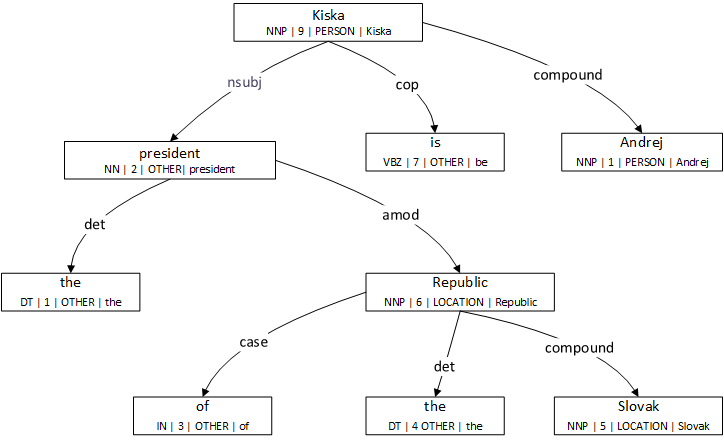
\includegraphics[scale=0.35]{tree_structure}\end{center}
	\caption[Stromová reprezentácia štruktúry]{Stromová reprezentácia štruktúry}\label{fig:tree_structure}
\end{figure}

%
% Reprezentácia vo vete
%
\ifthenelse {\boolean{bachelor}}
{
	\subsubsection{Reprezentácia vo vete}
}
{
	\subsection{Representation in sentence}
}
\label{subsubsection:structure_representation_in_sentence}
Reprezentácia vo vete taktiež reprezentuje vzťahy a prepojenia slov vo vete. Zo zobrazenia tejto reprezentácie sa dá jednoduchšie pochopiť celá štruktúra, keďže zobrazuje slová v pôvodnom poradí a celkovo vetu v originálnom formátovaní. Pre vetu \textit{,,The president of the Slovak Republic is Andrej Kiska.''} vyzerá \textit{reprezentácia vo vete} ako na~\imgref{fig:sentence_representation}.

\begin{figure}[H]
	\begin{center}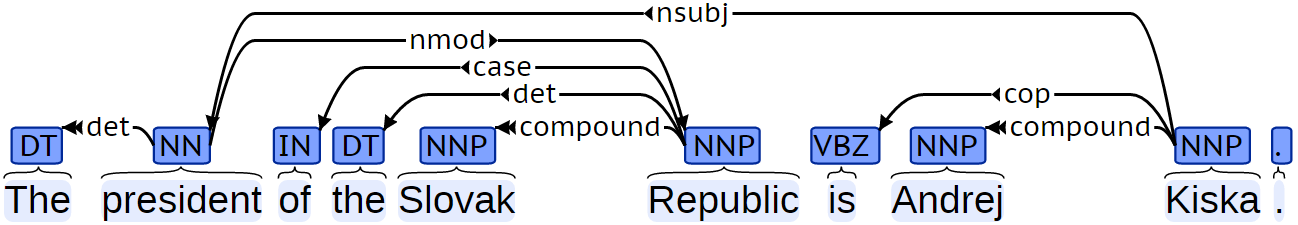
\includegraphics[scale=0.4]{kiska_full_sentence}\end{center}
	\caption[Reprezentácia štruktúry vo vete]{Reprezentácia štruktúry vo vete}\label{fig:sentence_representation}
\end{figure}

%
% Uchovávanie textov v databázach
%
\ifthenelse {\boolean{bachelor}}
{
	%\subsection{Subsection}
	\subsection{Uchovávanie textov v databázach}
}
{
	%\section{Subsection}
	\section{Uchovávanie textov v databázach}
}
\label{subsection:persisting_texts_in_db}
Text je špecifický údajový model s variabilnou štruktúrou, ktorý potrebujeme efektívne ukladať v databáze. Je nevyhnutné použiť vhodnú databázu, ktorá je prispôsobená na ukladanie textov. Databáza musí obsahovať vlastnosti, ktoré umožňujú jednoduché narábanie s dátami s variabilnou štruktúrou a nemajú prebytočnú spotrebu pamäti pri ich uchovávaní. Taktiež je potrebná podpora bezproblémového ukladanie, získavania, vyhľadávania a spracovania textov na úrovni databázy. Pri výbere vhodnej databázy sme prešli viacero alternatív.

%
% Relačné databázy
%
\ifthenelse {\boolean{bachelor}}
{
	%\subsection{Subsection}
	\subsubsection{Relačné databázy}
}
{
	%\section{Subsection}
	\subsection{Relačné databázy}
}
\label{subsubsection:relation_dbs}
%Relačné databázy boli dlhé roky populárnou a finančne nenáročnou voľbou pri tvorbe veľkých podnikateľských aplikácií. 
%Momentálne sú používané vo väčšine súčasných aplikácií a 
Relačné databázy pracujú spoľahlivo pri obmedzenom množstve dát~\cite{MongoDBvsMySQL2015}.
%Problém s relačným modelom relačných databáz nastáva, keď vzniká potreba aplikácie s obrovským množstvom dát. Menovite rozšíriteľnosť (angl. scalability) a schéme sa stávajú najväčším problémom relačných databáz~\cite{NoSQLDBvsRealtionDB}.
Pri potrebe aplikácie s obrovským množstvom dát sa rozšíriteľnosť (angl. scalability) a schéma stávajú problémom~\cite{NoSQLDBvsRealtionDB}.
Tento typ databáz ukladá dáta v tabuľkách zložených z riadkov a stĺpcov.
%Každý záznam (riadok) v tabuľke predstavuje zjednodušený objekt alebo vzťah z reálneho života. 
Výhodou relačných databáz je možnosť jednoduchého vytvorenia prispôsobeného pohľadu na dáta~\cite{Maier}. Z pohľadu ukladania textu, a celkovo dát s variabilnou štruktúrou, je nevýhoda relačných databáz v ťažko prispôsobiteľnej štruktúre.

%
% Textové databázy
%
\ifthenelse {\boolean{bachelor}}
{
	%\subsection{Subsection}
	\subsubsection{Textové databázy}
}
{
	%\section{Subsection}
	\subsection{Textové databázy}
}
\label{subsubsection:text_dbs}
%S rozmachom variácie dát v posledných rokoch sa začali objavovať a vznikať nerelačné databázy, aby pokryli požiadavky na nové aplikácie. Textové databázy sú druhom nerelačných databáz.
Textové databázy ukladajú dáta vo forme dokumentov, vďaka čomu ponúkajú vysoký výkon, horizontálnu rozšíriteľnosť a podporu pre ukladanie dát s variabilnou štruktúrou~\cite{NoSQLDBvsRealtionDB}. Uložené dokumenty môžu nadobúdať rôzne formáty, ako napríklad JSON, BSON, XML a BLOB, ktoré poskytujú veľkú flexibilnosť pre dáta. Každý záznam v takejto databáze preto môže mať inú štruktúru, napríklad počet alebo typ polí, čo šetrí úložným priestorom, keďže neobsahuje nepotrebné prázdne polia~\cite{NoSQLDBvsRealtionDB}.
%Dokumenty v databáze sú referencované kľúčom, ktorý môže byť reťazec, cesta, ale dokonca aj dokument~\cite{NoSQLDBvsRealtionDB}. 
%Dokumenty majú dynamickú schému, čo umožňuje vytvárať záznamy bez toho, aby bolo potrebné predtým definovať štruktúru. 
Dokumenty uľahčujú zmenu štruktúry záznamov jednoduchým pridaním, odstránením alebo zmenou typu poľa. Vďaka svojej štruktúre sú dokumenty ľahko namapovateľné na objekty z objektovo-orientovaných programovacích jazykov a odstraňujú tým potrebu pre použitie objektovo-relačnej mapovacej vrstvy. Dátovy typ dokument v textových databázach vyhovuje požiadavkám na databázu pre náš systém. Dokáže jednoducho narábať s dátami s variabilnou štruktúrou, bez nároku na prebytočnú pamäť a s dobrou rozšíriteľnosťou.

%Primárne využitie týchto databáz je v aplikáciách, ktoré potrebujú ukladať dáta, ktorých štruktúra je vopred neznáma alebo sa mení. Predstaviteľmi sú napríklad \textit{MongoDB} alebo \textit{CouchDB} databázy.

%
% Porovnanie a výber typu databázy
%
\ifthenelse {\boolean{bachelor}}
{
	%\subsection{Subsection}
	\subsubsection{Porovnanie a výber typu databázy}
}
{
	%\section{Subsection}
	\subsection{Porovnanie a výber typu databázy}
}
\label{subsubsection:compare_dbs}

Porovnávame textové a relačné databázy. V oboch kategóriách sme vybrali jedného z najväčších predstaviteľov danej kategórie. Za relačné databázy to je \textit{MySQL} a za textové databázy \textit{MongoDB}. Porovnanie poskytovaných prvkov porovnávaných databáz je v tabuľke~\fullref{table:features_of_mongodb}. 

\begin{table}[H]
	\centering
	\caption{Porovnanie poskytovaných prvkov}
	\label{table:features_of_mongodb}
	\begin{tabular}{|l|l|l|}
		\hline
		& \textbf{MySQL} & \textbf{MongoDB} \\ \hline
		Bohatý dátový model & Nie & Áno \\ \hline
		Dynamická štruktúra & Nie & Áno \\ \hline
		Dátové typy & Áno & Áno \\ \hline
		Lokálnosť dát & Nie & Áno \\ \hline
		Aktualizovanie polí & Áno & Áno \\ \hline
		Ľahké pre programátorov & Nie & Áno \\ \hline
		Komplexné transakcie & Áno & Nie \\ \hline
		Audit & Áno & Áno \\ \hline
		Auto-sharding & Nie & Áno \\ \hline
	\end{tabular}
\end{table}

\textit{Bohatý dátový model} (angl. Rich Data Model) je poskytovanie rozšírenej funkcionality dátovým modelom. Princípom \textit{dynamickej štruktúry} (angl. Dynamic Structure) je jednoduchá zmena štruktúru, pričom nemusí byť vôbec zadefinovaná, a každý záznam môže mať odlišnú štruktúru. \textit{Lokálnosť dát} (angl. Data Locality) znamená uchovávanie súvisiacich dát pokope. \textit{Aktualizovanie polí} umožňuje vykonávať nad poliami operácie, ako sú inkrementácia podľa špecifikovaného množstva, vynásobenie hodnotou, premenovanie, aktualizácia iba ak je hodnota väčšia alebo menšia ako špecifická hodnota a ďalšie. \textit{Audit} (angl. Auditing) je funkcionalita, ktorá umožňuje administrátorom a používateľom sledovať aktivity systému. \textit{Auto-sharding} zabezpečuje zabránenie poklesu priepustnosti operácií čítania a zapisovania pri náraste dát ukladaním dát automaticky na viacero strojov.

MongoDB má vlastnú konvenciu názvov svojich častí. Tie sa v niektorých prípadoch líšia s názvami relačných databáz. Rozdiely sú zobrazene v tabuľke~\fullref{table:names_of_mongodb}.

\begin{table}[H]
	\centering
	\caption{Porovnanie používaných pojmov~\cite{MongoDBvsMySQL2015}}
	\label{table:names_of_mongodb}
	\begin{tabular}{|l|l|}
		\hline
		\textbf{MySQL} & \textbf{MongoDB} \\ \hline
		Databáza & Databáza \\ \hline
		Tabuľka & Kolekcia \\ \hline
		Index & Index \\ \hline
		Riadok & BSON dokument \\ \hline
		Stĺpec & BSON pole (angl. field) \\ \hline
		Spojenie & Vnorené dokumenty a prepojenie \\ \hline
		Primárny kľúč & Primárny kľúč \\ \hline
		Zoskupenie & Agregácia \\ \hline
	\end{tabular}
\end{table}

Pri ukladaní textov a iných časti systému v databáze potrebujeme dynamickú štruktúru z dôvodu variability štruktúry ukladaných dát. Namapovanie dát na pevne stanovenú štruktúru a vzťahy relačných databáz by bolo veľmi náročné. Preto je výhodnejšie uchovávať dáta pokope v dynamickej štruktúre. Z bodov \textit{dynamická štruktúra} a \textit{lokálnosť dát} z tabuľky~\fullref{table:features_of_mongodb} jasne vidno, že pre tento účel je textová databáza vhodnejšia. \textit{Bohatý dátový model} je rovnako veľkou výhodou. V neposlednom rade \textit{MongoDB} automaticky podporuje \textit{sharding}, ktorý sa dá spraviť aj v databáze \textit{MySQL}, ale za cenu výkonnosti. Z týchto dôvodov sme sa rozhodli pre použitie textovej databázy v našom systéme.

%
% Ostatné databázové systémy
%%
%\ifthenelse {\boolean{bachelor}}
%{
%	%\subsection{Subsection}
%	\subsubsection{Ostatné databázové systémy}
%}
%{
%	\%section{Subsection}
%	\subsection{Ostatné databázové systémy}
%}
%\label{subsection:types_of_norelation_dbs}
%Okrem relačných a textových databáz existuje sme prešli ešte niekoľko druhov databáz.
%
%%
%% Kľúč - hodnota databázy
%%
%\ifthenelse {\boolean{bachelor}}
%{
%	%\subsection{Subsection}
%	\paragraph{Kľúč - hodnota databázy}
%}
%{
%	\%section{Subsection}
%	\subsubsection{Kľúč - hodnota databázy}
%}
%\label{subsubsection:key_value_db}
%%Nerelačné databázy typu kľúč - hodnota sú v svojej podstate celkom jednoduché, ale zároveň efektívne. Umožňujú používateľovi ukladať dáta ľubovoľne, kedže neobsahujú schémy. 
%Uložené dáta sa skladajú z dvoch častí. Prvá časť je kľuč a druhá časť je hodnota~\cite{NoSQLDBvsRealtionDB}, pričom kľúč je samo-generujúci string a hodnota môže byť takmer čokoľvek, od string, JSON cez BLOB až po obrázok~\cite{MongoDBvsMySQL2015}.
%%Kľúč - hodnota databázy sú veľmi podobné hašovacím tabuľkám, kde kľúč je indexom do tabuľky, pomocou ktorého používateľ môže pristúpiť k hodnote daného kľúču. Tento typ databáz uprednostňuje rozšíriteľnosť pred konzistenciou. Ponúka vysokú konkurenčnosť (angl. concurrency), rýchle vyhľadávanie a schopnosť uloženia veľkého množstva dát za cenu spojovacích a agregačných operácií. Taktiež 
%V tomto type databáz je veľmi náročné vytvoriť ľubovoľný pohľad na dáta z dôvodu chýbajúcej schémy~\cite{NoSQLDBvsRealtionDB}.
%
%%Najznámejšími predstaviteľmi tohto typu databáz sú \textit{Amazon DynamoDB} a \textit{RIAK}.
%
%%
%% Stĺpcové databázy
%%
%\ifthenelse {\boolean{bachelor}}
%{
%	%\subsection{Subsection}
%	\paragraph{Stĺpcové databázy}
%}
%{
%	\%section{Subsection}
%	\subsubsection{Stĺpcové databázy}
%}
%\label{subsubsection:column_db}
%Stĺpcové databázy musia mať preddefinovanú schému, v ktorej sú jednotlivé bunky záznamov zoskupené do kolekcie stĺpcov~\cite{MongoDBvsMySQL2015}.
%% Dáta nie sú ukladané do tabuliek, ale do masívne distribuovaných architektúr, s hlavným zámerom, aby agregácia dát mohla prebehnúť veľmi rýchlo s redukovaním I/O aktivity.
%%Tento typ databáz taktiež poskytuje veľkú rozšíriteľnosť v ukladaní dát.
%Najvhodnejšie je využívať stĺpcové databázy v analytických aplikáciách alebo aplikáciách, ktoré získavajú dáta pomocou metódy \textit{data mining}~\cite{NoSQLDBvsRealtionDB}.
%
%%
%% Grafové databázy
%%
%\ifthenelse {\boolean{bachelor}}
%{
%	%\subsection{Subsection}
%	\paragraph{Grafové databázy}
%}
%{
%	\%section{Subsection}
%	\subsubsection{grafové databázy}
%}
%\label{subsubsection:graph_db}
%%Grafové databázy su špeciálny typ databáz, v ktorých sú 
%Dáta sú uložené vo forme grafu. Graf pozostáva z vrcholov a hrán, pričom vrcholy predstavujú objekty a hrany reprezentujú vzťahy medzi nimi. Každý vrchol okrem iného obsahuje aj ukazovateľ na priľahlé vrcholy, čo umožňuje prechádzať obrovské množstvo dát rýchlejšie ako v relačných databázach~\cite{NoSQLDBvsRealtionDB}.
%
%%Údaje sa ukladajú v polo-štruktúrovanej forme, kde je kladený hlavný dôraz na prepojenia medzi dátami. Grafové databázy spĺňajú vlastnosť ACID a sú veľmi vhodné pre biometrické aplikácie alebo aplikácie sociálnych sietí. Hlavným predstaviteľom grafových databáz je \textit{Neo4j}~\cite{NoSQLDBvsRealtionDB}.
%
%%
%% Objektovo orientované databázy
%%
%\ifthenelse {\boolean{bachelor}}
%{
%	%\subsection{Subsection}
%	\paragraph{Objektovo orientované databázy}
%}
%{
%	\%section{Subsection}
%	\subsubsection{Objektovo orientované databázy databázy}
%}
%\label{subsubsection:object_oriented_db}
%Objektovo orientované databázy ukladajú dáta vo forme objektov, rovnako ako sú údaje reprezentované v objektoch v objektovo orientovaných programovacích jazykoch (OOP). Tieto databázy podporujú všetky vymoženosti OOP, ako enkapsulácia, polymorfizmus, ale aj dedenie. Objektovo orientované databázy robia moderný vývoj softvéru jednoduchším~\cite{NoSQLDBvsRealtionDB}.

%
% Zhrnutie aplikácií na spracovanie prirodzeného jazyka
%
%\ifthenelse {\boolean{bachelor}}
%{
%	%\subsection{Subsection}
%	\subsubsection{Zhrnutie}
%}
%{
%	%\section{Subsection}
%	\section{Zhrnutie}
%}
%\label{subsection:design_shrnutie}
%NOSQL databáza je narozdiel do RDBMS modelu (Relation Data Base Management System)
%navrhnutá, tak aby bola jednoducho rozšíriteľná so zväčšovaním dát. Väčšina NOSQL databáz odstránila niektoré nepotrebné prvky RDBMS modelov, čím sa stali podstatne ľahšími a efektívnejšími. Toto na druhej strane spôsobilo, že NOSQL model negarantuje vlastnosti ACID (Atomicity, Consistency, Isolation, Durability), ale naopak garantuje vlastnosti BASE (Basically Available, Soft state, Eventula Consistency)~\cite{NoSQLDBvsRealtionDB}.
%
%Nerelačné databázy neukladajú údaje v tabuľkách a nemajú fixnú schému. Tieto vlastnosti im umožňujú jednoducho spracovávať neštruktúrované dáta, ako sú dokumenty, e-maily a mnoho ďalších~\cite{MongoDBvsMySQL2015}. Preto majú čím ďalej, tým viac využití.
%
%Existuje hneď niekoľko prípadov, kedy je lepšie použiť nerelačnú databázu namiesto relačnej databázy. Keď je potrebné, aby aplikácia dokázala spracovávať rôzne typy a tvary dát alebo pri potrebe spravovať aplikáciu efektívnejšie pri rozširovaní, je rozhodne výhodnejšie použiť nerelačnú databázu. Niektoré databázy, ako napríklad textová databáza MongoDB uľahčuje vývoj aplikácií, keďže jeho dokumentová štruktúra dát je jednoducho namapovateľná na moderné, objektovo-orientované programovacie jazyky a tým pádom nie je potreba využívať komplexnú objektovo-relačnú mapovaciu vrstvu, ktorá je nutná pri použití relačných databáz na prevod objektov z programovacie jazyka na perzistentné objekty v databáze. Všeobecne je omnoho ľahšie rozšíriť schému / model nerelačnej databázy ako rozširovať schému relačnej databázy.
%
%V systéme potrebujeme ukladať v databáze texty a informácie o nich. Počet viet, slov, vzťahov je pre každý text odlišný a preto nedokážeme vopred definovať efektívnu schému na ukladanie týchto dát. Textové databázy, so svojou dynamickou a ľahko upraviteľnou štruktúrou, sú na tento účel ideálne, pričom ukladanie textov v tabuľkách by bolo náročne, navyše relačné databázy nemajú predvolené podporované vyhľadávania v štruktúrach ako text. MongoDB (viď.~\fullref{subsection:mongodb}) je vyspelá, dokumentová databáza zahrňajúca všetku funkcionalitu, ktorú potrebujeme.

%
% Návrh uchovávania textov v databázach
%
\ifthenelse {\boolean{bachelor}}
{
	%\subsection{Subsection}
	\subsection{Návrh uchovávania textov v databázach}
}
{
	%\section{Subsection}
	\section{Návrh uchovávania textov v databázach}
}
\label{subsection:our_design_persisting_data}
Ukladané dáta sa dajú rozdeliť do niekoľkých samostatných kolekcií. Sú to:

\begin{my_itemize}
	\myitem rules,
	\myitem sentences,
	\myitem notes
	\myitem structures,
	\myitem articles,
	\myitem and rules.
\end{my_itemize}
	
Prepojenia medzi jednotlivými kolekciami sú zobrazené na~\imgref{fig:db_schema}. Nasledujúcich časti opisujú stručne každú kolekciu. Všetky kolekcie obsahujú okrem polí špecifických pre danú kolekciu, aj polia časových značiek označujúcich vytvorenie a aktualizáciu záznamu.

\begin{figure}[H]
	\begin{center}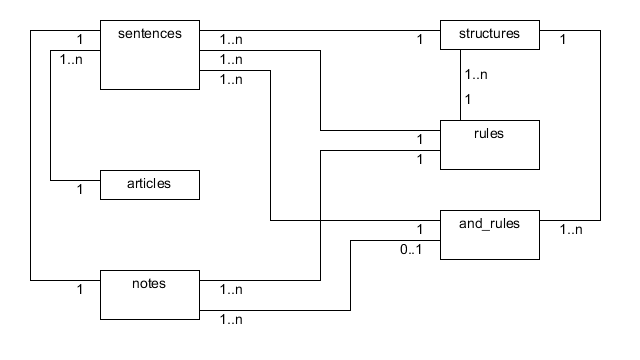
\includegraphics[scale=0.60]{db_schema}\end{center}
	\caption[Databázový model]{Databázový model}\label{fig:db_schema}
\end{figure}

%
% Kolekcia texts
%
\ifthenelse {\boolean{bachelor}}
{
	%\subsection{Subsection}
	\subsubsection{Kolekcia articles}
}
{
	%\section{Subsection}
	\subsection{Kolekcia articles}
}
\label{subsubsection:collection_articles}
V kolekcii \textit{articles} sa ukladajú spracovávané texty. 

Kolekcia obsahuje textové pole \textit{text} na uloženie textu v pôvodnom tvare. Model kolekcie \textit{articles} je zobrazený na~\imgref{fig:articles_collection_model}.

\begin{figure}[H]
	\begin{center}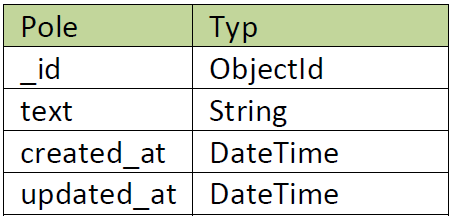
\includegraphics[scale=0.60]{articles_model}\end{center}
	\caption[Model kolekcie articles]{Model kolekcie articles}\label{fig:articles_collection_model}
\end{figure}

%
% Kolekcia notes
%
\ifthenelse {\boolean{bachelor}}
{
	%\subsection{Subsection}
	\subsubsection{Kolekcia notes}
}
{
	%\section{Subsection}
	\subsection{Kolekcia notes}
}
\label{subsubsection:collection_notes}
Kolekcia \textit{notes} uchováva vytvorené poznámky z viet.

Obsahuje textové pole \textit{text} s hodnotou poznámky a dve referencujúce polia. Jedno sa odkazuje do kolekcie \textit{rules} na pravidlo, ktoré bolo použité na vytvorenie poznámky. Druhé referencuje použité and\hyph pravidlo v kolekcií \textit{and\textunderscore rules}. Toto pole môže byť prázdne, ak sa and\hyph pravidlo pri vytváraní poznámky nepoužilo. Na~\imgref{fig:notes_collection_model} je vyobrazený model kolekcie \textit{notes}.

\begin{figure}[H]
	\begin{center}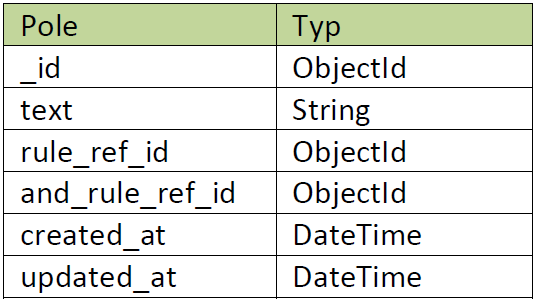
\includegraphics[scale=0.60]{notes_model}\end{center}
	\caption[Model kolekcie notes]{Model kolekcie notes}\label{fig:notes_collection_model}
\end{figure}

%
% Kolekcia sentences
%
\ifthenelse {\boolean{bachelor}}
{
	%\subsection{Subsection}
	\subsubsection{Kolekcia sentences}
}
{
	%\section{Subsection}
	\subsection{Kolekcia sentences}
}
\label{subsubsection:collection_sentences}
V následujúcej kolekcii \textit{sentences} sa ukladajú spracované vety aj s informáciami o článku, pravidlách a poznámke.

Kolekcia sa skladá z textového polia \textit{text} uchovávajúce hodnotu vety a piatich referencujúcich polí \textit{article\textunderscore ref\textunderscore id}, \textit{structure\textunderscore ref\textunderscore id}, \textit{rule\textunderscore ref\textunderscore id}, \textit{and \textunderscore rule\textunderscore ref\textunderscore id} a \textit{note\textunderscore id}. \textit{Article\textunderscore ref\textunderscore id} odkazuje na článok z kolekcie \textit{articles}, ktorého súčasťou je daná veta. Pole \textit{structure\textunderscore ref\textunderscore id} odkazuje do kolekcie \textit{structures}, ktoré reprezentuje štruktúru vety. Nasledujúce polia \textit{rule\textunderscore ref\textunderscore id} a \textit{and\textunderscore rule\textunderscore ref\textunderscore id} odkazujú na použité pravidlo a and\hyph pravidlo pri spracovávaní vety, v tomto poradí. Pole \textit{note\textunderscore ref\textunderscore id} odkazuje na poznámku z kolekcie \textit{notes}, ktorá bola vytvorená z vety.

Model tejto kolekcie je načrtnutý na~\imgref{fig:sentences_collection_model}.

\begin{figure}[H]
	\begin{center}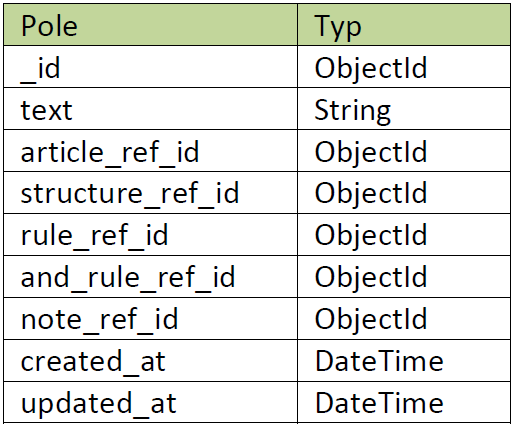
\includegraphics[scale=0.60]{sentences_model}\end{center}
	\caption[Model kolekcie sentences]{Model kolekcie sentences}\label{fig:sentences_collection_model}
\end{figure}

%
% Kolekcia structures
%
\ifthenelse {\boolean{bachelor}}
{
	%\subsection{Subsection}
	\subsubsection{Kolekcia structures}
}
{
	%\section{Subsection}
	\subsection{Kolekcia structures}
}
\label{subsubsection:collection_structures}
V kolekcií \textit{structures} sú uložené štruktúry viet a pravidiel. Štruktúra je zložená hlavne zo závislostí, tokenov, názvoslovných značiek, indexov a iné.

Kolekcia sa skladá z jedného pola \textit{structure\textunderscore data}. Toto pole je zoznam dokumentov, obsahujúcich vyššie spomenuté údaje. Dokument v tomto zozname obsahuje textové pole \textit{relation\textunderscore name} s názvom vzťahu závislosti a zoznam dokumentov závislostí \textit{dependencies} s týmto názvom vzťahu. Dokument v zozname \textit{dependencies} sa skladá z polí \textit{governor} a \textit{dependent} typu dokument, celočíselného pola \textit{position} uchovávajúceho pozíciu závislosti vo vete alebo poznámke, \textit{comparison\textunderscore type}, ktoré je celočíselnou reprezentáciou typu porovnania a poľa \textit{token\textunderscore type}, ktoré je taktiež celočíselnou reprezentáciou typu tokenu. Dokumenty polí \textit{governor} a \textit{dependent} obsahujú údaje o prislúchajúcich tokenoch závislosti. V textovom poli \textit{POS} sa ukladá značka slovného druhu, pole \textit{index} uchováva index tokenu vo vete, \textit{ner} je textové pole reprezentujúce názvoslovnú entitu tokenu a v poli \textit{lemma} je textová reprezentácia lemy tokenu.

Celý model kolekcie je zobrazený na~\imgref{fig:structures_collection_model}.

\begin{figure}[H]
	\begin{center}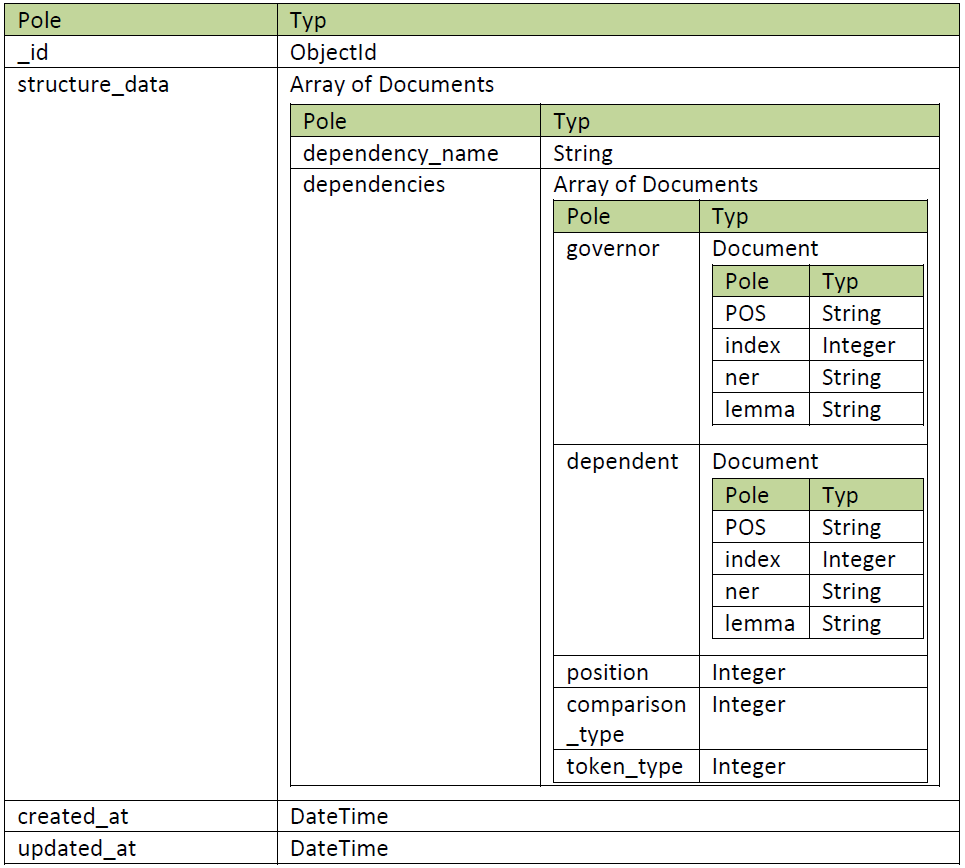
\includegraphics[scale=0.53]{structure_model}\end{center}
	\caption[Model kolekcie structures]{Model kolekcie structures}\label{fig:structures_collection_model}
\end{figure}

%
% Kolekcia rules
%
\ifthenelse {\boolean{bachelor}}
{
	%\subsection{Subsection}
	\subsubsection{Kolekcia rules}
}
{
	%\section{Subsection}
	\subsection{Kolekcia rules}
}
\label{subsubsection:collection_rules}
\textit{Rules} je kolekcia, do ktorej sa ukladajú pravidla na vytvorenie poznámok z viet. Vďaka databázovému modelu na~\imgref{fig:db_schema} a prepojeniam medzi kolekciami je táto kolekcia minimalistická.

Skladá sa z dvoch polí. Pole \textit{sentence\textunderscore terminators} je zoznam čísel, ktoré reprezentujú konce viet v poznámke. Referencujúce pole \textit{structure\textunderscore ref\textunderscore id} odkazuje do kolekcie \textit{structures} na štruktúru, ktorou sa má prípadná veta spracovať. Model kolekcie \textit{rules} je vyjadrený~\imgref{fig:rules_collection_model}.

Pole \textit{sentence\textunderscore terminators} zväčša obsahuje jeden záznam. Napríklad pri vete \textit{,,The president of the Slovak Republic is Andrej Kiska.''} a poznámke z tejto vety v tvare \textit{,,President is Kiska.''} bude obsahovať jeden záznam: 3. Číslo 3, lebo koniec vety, v tomto prípade bodka, sa nachádza na tretej pozícií spomedzi tokenov vo vete. Číslovanie pozícií začína od nuly. V prípade ak veta je súvetie, zložené z viacerých jednoduchých viet, môže pole \textit{sentence\textunderscore terminators} obsahovať viacero záznamov, ak napríklad chceme z každej jednoduchej vety súvetia získať zjednodušenú vetu a vytvoriť tak zloženú poznámku, skladajúcu sa zo zjednodušených viet.

\begin{figure}[H]
	\begin{center}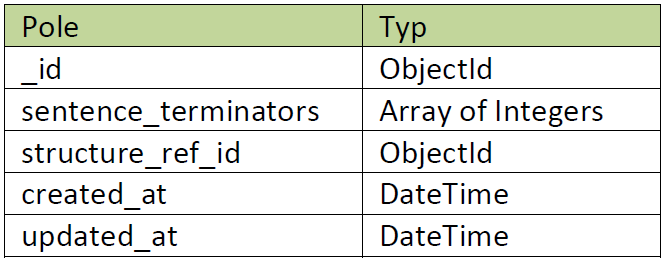
\includegraphics[scale=0.60]{rules_model}\end{center}
	\caption[Model kolekcie rules]{Model kolekcie rules}\label{fig:rules_collection_model}
\end{figure}

%
% Kolekcia and_rules
%
\ifthenelse {\boolean{bachelor}}
{
	%\subsection{Subsection}
	\subsubsection{Kolekcia and rules}
}
{
	%\section{Subsection}
	\subsection{Kolekcia and rules}
}
\label{subsubsection:collection_and_rules}
Posledná kolekcia uchováva pravidlá pre spracovanie vety a vytvorenie viacnásobnej poznámky z vety. Táto kolekcia je veľmi podobná kolekcií \textit{rules} a obsahuje rovnaké polia doplnené o ďalšie špecifické pole.

Špecifické pole, o ktoré je kolekcia rozšírená oproti kolekcií \textit{rules} je celočíselné pole \textit{set\textunderscore position}. Toto pole uchováva pozíciu množiny vo viacnásobnej poznámke. Model kolekcie je vyobrazený na~\imgref{fig:and_rules_collection_model}.

\begin{figure}[H]
	\begin{center}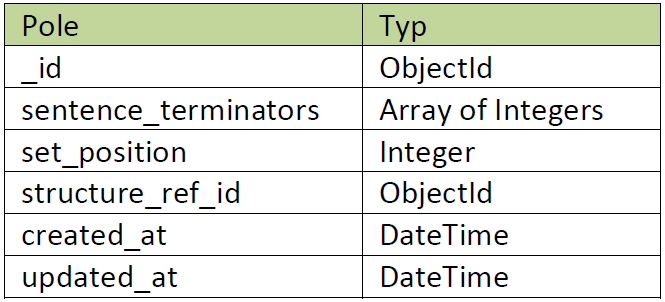
\includegraphics[scale=0.60]{and_rules_model}\end{center}
	\caption[Model kolekcie and rules]{Model kolekcie and rules}\label{fig:and_rules_collection_model}
\end{figure}

%Dáta sú v MongoDB databáze uložené v binárnom JSON formáte. Na ukážke~\fullref{code:collection_rules_data_example} je zobrazená časť uložených údajov o pôvodnej vete. Ukážka celého záznamu pre vetu ,,The president of the Czech Republic is Milos Zeman.'' je priložená v prílohe~\fullref{appendix:db_entry_full_example}.
%\\
%\begin{lstlisting}[language = json, caption={Ukážka dát kolekcie rules}, label = {code:collection_rules_data_example}]
%{  
%	"originalDependencies" : [  
%		{  
%			"dependencyName" : "det",
%			"dependencies" : [  
%				{  
%					"governor" : {  
%						"pos" : "NN",
%						"index" : 2
%					},
%					"dependent" : {  
%						"pos" : "DT",
%						"index" : 1
%					},
%					"position" : 0
%				},
%				{ ... }
%			]
%		}
%	]
%}
%\end{lstlisting}

%
% Kolekcie zhrnutie
%
\ifthenelse {\boolean{bachelor}}
{
	\subsubsection{Zhrnutie kolekcií}
}
{
	\subsection{Zhrnutie kolekcií}
}
\label{subsubsection:collections_summary}
Pri návrhu databázového modelu a kolekcií sme vychádzali z princípu jednoduchých kolekcií so zoskupením súvisiacich dát a oddelenia ich od zvyšku. Vďaka využívaniu viacerých, medzi sebou prepojených, kolekcií sme zabezpečili neduplikovanie dát, jednoduché vyhľadanie, napríklad viet ku článku a iné. Okrem toho nám tento model umožňuje ďalšiu funkcionalitu, ako napríklad aplikovanie jedného pravidla na viacero viet so zhodnou štruktúrou. Oddelenie dát do samostatných kolekcií nám uľahčuje aj prípadne neskoršie rozšírenie databázového modelu alebo zmenu konkrétnych kolekcií. Taktiež uľahčuje prípadné klastrovanie databázy, ak by bolo nutné, keďže každá kolekcia by mohla byť na samostatnom serveri.

%
% Zhrnutie
%
\ifthenelse {\boolean{bachelor}}
{
	%\subsection{Subsection}
	\subsection{Zhrnutie}
}
{
	%\section{Subsection}
	\section{Summary}
}
\label{subsection:design_summary}
Systém dokáže vytvoriť poznámku z viet na základe pravidla. Pravidlo je tvorené primárne zo závislostí, značiek slovných druhov a typov názvoslovných entít. Závislostí majú viacero využití pri tvorbe poznámok, hlavné z nich sú jednoznačná identifikácia informácie a pravidlo závisle od štruktúry vety. Z toho vyplýva, že pravidlo je aplikovateľné na viacero viet s rovnakou štruktúrou. Štruktúru si vieme reprezentovať stromom alebo priamo vo vete. Informácie o spracovaných článkoch, vetách a vytvorených poznámkach a pravidlách sa ukladajú do textovej databázy s dôkladne navrhnutým modelom.